\documentclass[12pt,a4paper,twoside]{book}

\usepackage[utf8]{inputenc}
\usepackage[english]{babel}

\usepackage[a4paper,inner=3.5cm,outer=2.5cm]{geometry}
\usepackage{parskip}
\usepackage{indentfirst}

\usepackage{graphicx}
\usepackage{float}
\usepackage{booktabs}
\usepackage{tabularx}
\usepackage{multirow}

\usepackage{natbib}
\bibliographystyle{ieeetr}
\setcitestyle{super,open={[},close={]}}

\usepackage{hyperref}

\usepackage{amsmath}
\usepackage{bm}

\usepackage[titletoc,title,toc,page]{appendix}
\usepackage{chngcntr}
\counterwithin{table}{chapter}
\usepackage[capitalize,noabbrev]{cleveref}

\usepackage{newlfont}
\usepackage{fancyhdr}
\usepackage{soul}
\usepackage{xcolor}
\usepackage{hyphenat}
\hyphenation{mate-mati-ca recu-perare}

\usepackage{listings}
\usepackage{verbatim}

\usepackage{tikz}
\usepackage{lscape}

\usepackage{tcolorbox}
\tcbuselibrary{skins, breakable}

\usepackage[font=footnotesize,labelfont=bf]{caption}

\newcommand{\rom}[1]{\uppercase\expandafter{\romannumeral #1\relax}}

\usepackage{pdfpages}

\lstset{
  aboveskip=1em,
  breaklines=true,
  captionpos=b,
  escapeinside={\%*}{*)},
  frame=single,
  numbers=left,
  numbersep=15pt,
  numberstyle=\tiny,
  basicstyle=\ttfamily\footnotesize
}

\definecolor{maroon}{cmyk}{0, 0.87, 0.68, 0.32}
\definecolor{halfgray}{gray}{0.55}
\definecolor{ipython_frame}{RGB}{207, 207, 207}
\definecolor{ipython_bg}{RGB}{247, 247, 247}
\definecolor{ipython_red}{RGB}{186, 33, 33}
\definecolor{ipython_green}{RGB}{0, 128, 0}
\definecolor{ipython_cyan}{RGB}{64, 128, 128}
\definecolor{ipython_purple}{RGB}{170, 34, 255}
\definecolor{outputcellbg}{RGB}{248,248,248}

\lstdefinelanguage{Python}{
    morekeywords={access,and,break,class,continue,def,del,elif,else,except,exec,finally,for,from,global,if,import,in,is,lambda,not,or,pass,print,raise,return,try,while},
    morekeywords=[2]{abs,all,any,basestring,bin,bool,bytearray,callable,chr,classmethod,cmp,compile,complex,delattr,dict,dir,divmod,enumerate,eval,execfile,file,filter,float,format,frozenset,getattr,globals,hasattr,hash,help,hex,id,input,int,isinstance,issubclass,iter,len,list,locals,long,map,max,memoryview,min,next,object,oct,open,ord,pow,property,range,raw_input,reduce,reload,repr,reversed,round,set,setattr,slice,sorted,staticmethod,str,sum,super,tuple,type,unichr,unicode,vars,xrange,zip,apply,buffer,coerce,intern},
    sensitive=true,
    morecomment=[l]\#,
    morestring=[b]',
    morestring=[b]",
    morestring=[s]{'''}{'''},
    morestring=[s]{"""}{"""},
    identifierstyle=\color{black}\ttfamily,
    commentstyle=\color{ipython_cyan}\ttfamily,
    stringstyle=\color{ipython_red}\ttfamily,
    keepspaces=true,
    showspaces=false,
    showstringspaces=false,
    rulecolor=\color{ipython_frame},
    frame=single,
    numbers=left,
    numberstyle=\tiny\color{halfgray},
    backgroundcolor=\color{ipython_bg},
    basicstyle=\scriptsize,
    keywordstyle=\color{ipython_green}\ttfamily,
}

\newtcolorbox{definition}[1][]{
    enhanced,
    breakable,
    colback=white,
    colframe=maroon,
    arc=2pt,
    boxrule=0.8pt,
    left=10pt,
    right=10pt,
    top=8pt,
    bottom=8pt,
    fonttitle=\bfseries,
    coltitle=white,
    title=Definition,
    #1
}

\newtcolorbox{example}[1][]{
    enhanced,
    breakable,
    colback=white,
    colframe=gray,
    arc=2pt,
    boxrule=0.8pt,
    left=10pt,
    right=10pt,
    top=8pt,
    bottom=8pt,
    fonttitle=\bfseries,
    coltitle=white,
    title=Example,
    #1
}

\newcommand\ownfootnote[1]{%
  \begin{NoHyper}
  \renewcommand\thefootnote{}\footnote{#1}%
  \addtocounter{footnote}{-1}%
  \end{NoHyper}
}

\begin{document}
\pagestyle{empty}
\newgeometry{left=2cm, right=2cm}
\begin{titlepage}
\begin{center}
    {{\Large{\textsc{Alma Mater Studiorum $\cdot$ Università di Bologna}}}}
    \rule[0.1cm]{\textwidth}{0.1mm}
    \rule[0.5cm]{\textwidth}{0.6mm}\\
    {\small{\bf Second Cycle Degree\\
    Artificial Intelligence}}
\end{center}

\vspace{45mm}

\begin{center}
    \textbf{Fundamentals of Artificial Intelligence and Knowledge Rapresentation}
\end{center}

\vspace{60mm}
\par
\noindent
\begin{minipage}[t]{0.04\textwidth}
~
\end{minipage}
\begin{minipage}[t]{0.4\textwidth}
{{\textbf{Student:}\\
Matteo Canghiari}}
\end{minipage}
\begin{minipage}[t]{0.04\textwidth}
~
\end{minipage}

\vspace{30mm}

\begin{center}
    {\large{\bf Academic Year 2025/2026}}
\end{center}
\end{titlepage}

\restoregeometry

\pagestyle{empty}
\newpage~\newpage
\thispagestyle{empty}

\clearpage
\pagenumbering{arabic}
\pagestyle{plain}

\chapter{Acting under uncertainty}
Many AI problems can be solved by exploring the \textbf{solution space}. A solution space is a set of all the sequences of actions that an agent can apply. The agent examines all
the possible sequences of actions and chooses the best one. The goal is to reach the solution starting from a \textbf{initial state}. The process of trying different sequences
is called \textbf{search}. \vspace{3.5pt}

Usually, it's useful to think about the \textbf{search} process as a \textbf{search tree}, where:
\begin{itemize}
    \renewcommand{\labelitemi}{-}
    \item The initial state corresponds to the \textbf{root} of the tree.
    \item Each branch that makes up the tree defines the \textbf{action} that can performed by the current node.
    \item The nodes represent the subsequent reachable states. However, a certain node can be a \textbf{leaf node}. A leaf node is a new state to expand, a solution or a dead-end.
\end{itemize}
Previously, we said that a solution is a sequence of actions, so we need to define two main operations that allow us to build a sequence. We do this by \textbf{expanding}
the current state, applying each possible action to the current node, \textbf{generating} a new set of states\footnote{Every time we expand the current node, new state are generated.}.
Generally, the set of all leaf nodes available for expansion at any given point is called \textbf{frontier} or \textbf{fringe}. The process of expanding nods continues until
either a solution is found or there are no more states to expand. \vspace{3.5pt}

Finally, concluding this first introduction, we say that all the search algorithms are named \textbf{search strategies}, and typically they all share the same structure, varying
by the way they choose which state needs to be expand.
\label{c_1}

\section{Basic probability notation}
Every search strategy uses different kind of data structures to keep in mind how the search tree was built. Each node of the tree corresponds to a data structure, containing:
\begin{itemize}
    \renewcommand{\labelitemi}{-}
    \item State: the state in the state space.
    \item Parent: the node that generated this node.
    \item Action: the action taken by the parent to generate the node.
    \item Depth: defining how deep is the node, in which level it belongs to.
    \item Path-Cost: the cost of the path from the initial state to this node, usually denoted by $g(n)$.
\end{itemize}
Now that we have nodes, we need somewhere to put them. The fringe needs to be stored in such a way that the search algorithm can easily choose the next node to expand. The 
appropriate data structure is a \textbf{queue}. It can be a \textbf{FIFO}, \textbf{LIFO} or a \textbf{priority queue}\footnote{We remember that: 
    \begin{itemize}
        \setlength{\itemsep}{0pt}
        \renewcommand{\labelitemi}{-}
        \item LIFO queues pop the newest element.
        \item FIFO queues pop the oldest element.
        \item Priority queues pop the element with the highest priority.
    \end{itemize}
}.
\label{s_1_1}

\section{Inference using full joint distribution}
This paragraph describes a new method to retrieve informations from data, named \textbf{probabilistic inference}.
It allows the computation of conditional probabilities for query propositions by given evidence.
Starting from an example is defined the \textbf{full joint distribution} as the knowledge base from which answers to all questions.
\begin{example}
  e.g. (\textit{Toothache, Cavity, Catch}) is just a domain consisting of three Boolean variables. \textit{Catch} condition occurs when the dentist's steel probe catches in the tooth. Based on the domain, the \textbf{full joint distribution} seems like this:
  \begin{center}
        \begin{table}[H]
            \centering
            \begin{tabular}{|c|c|c|c|c|}
                \hline
                \multicolumn{1}{|c|}{} & \multicolumn{2}{|c|}{\it toothache} & \multicolumn{2}{|c|}{\it $\neg$toothache} \\
                \hline
                \it & \it catch & \it $\neg$catch & \it catch & \it $\neg$catch \\
                \it cavity & 0.108 & 0.012 & 0.072 & 0.008 \\
                \it $\neg$cavity & 0.016 & 0.064 & 0.144 & 0.576 \\
                \hline
            \end{tabular}
            \caption{Full joint distribution of Toothache, Cavity and Catch}
            \label{t_1_2}
        \end{table}
    \end{center}
    The equation 
    \begin{center}
        $P(\phi) = \sum_{\omega:\omega\models\phi}P(\omega)$
    \end{center}
    gives a direct way to calculate probabilities of any assertions, summing up all the possible worlds that satisfy the original proposition. \vspace{3.5pt}

    e.g. $P(toothache) = 0.108 + 0.012 + 0.016 + 0.064 = 0.2$ 

    e.g. $P(cavity \vee toothache) = 0.108 + 0.012 + 0.072 + 0.008 + 0.016 + 0.064 = 0.28$

    It's also possible compute conditional probabilities: \vspace*{3.5pt}

    e.g. $P(\neg cavity|toothache) = \frac{P(\neg cavity \land toothache)}{P(toothache)} = \frac{0.016 + 0.064}{0.2} = 0.4$ \vspace{3.5pt}

    Notice that in this calculation the term $P(toothache)$ remains constant, no matter which value of \textit{Cavity} is computed. In fact, it can be viewed as a \textbf{normalization constant} $(\alpha)$ for the whole distribution $\mathbf{P}(Cavity|toothache)$, ensuring that the positive and negative case sum up to one, as the second probability axiom requires. \vspace*{7pt}

    $\mathbf{P}(Cavity|toothache) = \alpha\mathbf{P}(Cavity, toothache)$ \\
    $= \alpha[\mathbf{P}(Cavity, toothache, catch) + \mathbf{P}(Cavity, toothache, \neg catch)]$ \\
    $= \alpha[\langle0.108, 0.016\rangle + \langle0.012, 0.064\rangle]$ \\
    $= \alpha\langle0.12, 0.08\rangle = \langle0.6, 0.4\rangle$
\end{example}
\begin{definition}
    The first probability calculated $P(toothache)$ is called \textbf{marginalization}, or more simply \textbf{summing out}, because it sums up the probabilities for each possible value of the other variables.
\end{definition}
\begin{definition}
    The second one $P(\neg cavity|toothache)$ is named \textbf{conditioning}, a variant of marginalization that involves conditional probabilities instead of joint probabilities.
\end{definition}
\begin{definition}
    From the example, it's possible to extract a general inference procedure. Let \textbf{Y} be the query variables. Let \textbf{E} be the list of evidence variables, let \textbf{e} be the list of observed values for them, and let \textbf{H} be the unobserved variables. The \textbf{probability query} $\mathbf{P}(Y|\mathbf{e})$ defines the posterior joint distribution of a set of \textbf{query variables Y} given specific values \textbf{e} for some \textbf{evidence variables E}: \vspace{3.5pt}
    \begin{center}
        $\mathbf{P}(Y|e) = \alpha\mathbf{P}(Y, E=e) = \alpha\sum_{h}\mathbf{P}(Y, E=e, H=h)$
    \end{center}
\end{definition}
The full joint distribution can answer probabilistic queries for discrete variables, but only for small domains. It does not scale well: for a domain described by \textit{n} Boolean variables, it requires an input table of size \textit{$O(2^n)$} and takes \textit{$O(2^n)$} time to process a question. The full joint distribution in tabular form is just not a practical tool for building reasoning systems.
\label{s_1_2}

\chapter{Independence}
This chapter covers several search strategies that come under the heading of \textbf{non-informed strategies}. The term \textit{non-informed} means that the strategies have no 
additional knowledge about the domain; all they can do is generate successors and distinguish a goal state from a non-goal state. We introduce five non-informed search strategies:
\begin{itemize}
    \renewcommand{\labelitemi}{-}
    \item BFS.
    \item Uniform-cost search.
    \item DFS.
    \item DFS with limited depth.
    \item Iterative deepening.
\end{itemize}
\label{c_2}

\section{Bayes' rule}
\textbf{Breadth-first search} is a simple strategy in which the root node is expanded first, then all the successors of the root node are expanded next, and so on; until it is
found the goal-state or the goal-node. \vspace{3.5pt}

At algorithmic level, this is achieved very simply using a FIFO queue for the fringe, so the oldest node will be the first expanded. Before generating, so creating new states,
the goal-test is applied to the \textbf{shallowest} node. \vspace{3.5pt}

This strategy ensures \textbf{completeness}, but the \textbf{shallowest} goal node is not necessary the \textbf{optimal} one. BFS can be optimal if all the actions have the same 
path-cost. In addition, breadth-first search seems to take a quite huge of time and memory. Suppose a search tree where every node has $b$ successors. The root node generates
$b$ nodes at the first level, each of which generates $b$ more successors, for a total of $b^2$ nodes. Now if we consider that the goal-node has $d$ depth, in the worst case 
the total number of nodes generated is \vspace{3.5pt}
\begin{center}
    $b + b^2 + b^3 + \dots = O(b^d)$.
\end{center} \vspace{3.5pt}
This complexity is the same for both time and memory. As the time complexity, the memory takes into account every node expanded inside the \textbf{explored set} to avoid
\textbf{loopy path}; the space complexity grows exponentially with the number of $b$ successors and the depth $d$ of the goal node. The problem of memory seems to be the most serious. \vspace{3.5pt}

In general, any exponential complexity seems to be scary, and in this case uninformed strategies cannot solve massive problems.
\label{s_2_1}

\section{Bayes' rule: a simple case study}
The previous paragraph noted the importance of absolute and conditional independence relationships in simplifying probabilistic representation.
This section introduces a systematic way to represent such relationships in the form of \textbf{Bayesian networks}.
We define the syntax and semantics of these networks and show how they can be used to capture uncertain knowledge. \vspace{7pt}

A Bayesian network is a simple graphical notation for conditional independence assertions and hence for a compact specification of full joint distribution.
The Bayesian network's syntax is composed by:
\begin{enumerate}
    \item Each node corresponds to a random variable.
    \item A set of directed links or arrows connects pairs of nodes.
    \item Each node $X_i$ has a conditional probability distribution $\mathbf{P}(X_i|Parents(X_i))$, that quantifies the effect of the parents on the node.
\end{enumerate}
\begin{example}
    i.e. Topology of network encodes conditional independence assertions: \vspace{3.5pt}
    \begin{center}
        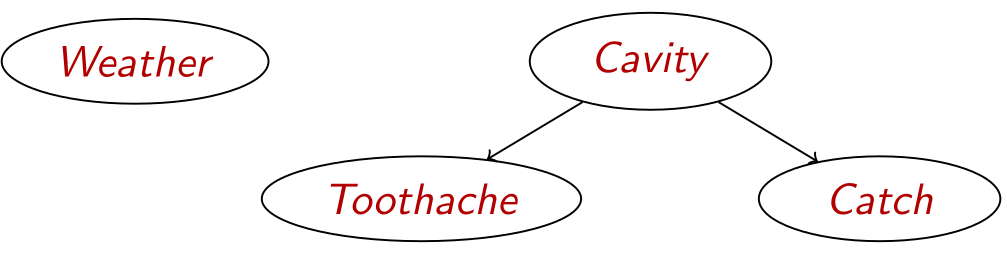
\includegraphics[width=0.6\textwidth]{img/img2.png}
    \end{center} \vspace{3.5pt}
    \begin{itemize}
        \renewcommand{\labelitemi}{-}
        \item Weather is independent of the other variables\footnote{Formally, the absolute or conditional independence is indicated by the absence of a link between nodes.}.
        \item Toothache and Catch are conditionally independent given Cavity\footnote{The intuitive meaning of an arrow is typically that X has a direct influnce on Y, which suggests that causes should be parents of effects.}.
    \end{itemize}
\end{example}
\begin{example}
    i.e. I'm at work, neighbor John calls to say my alarm is ringing, but neighbor Mary doesn't call. Sometimes it's set off by minor earthquakes. Is there a burglar? \vspace{3.5pt}

    The random variables are: \it Burglar, Earthquake, Alarm, MaryCalls, JohnCalls \footnote{The network topology reflects \textbf{causal} knowledge, from the causes nodes we define the effects nodes.}\footnote{For each node the conditional distribution are shown as a \textbf{conditional probability table}, or simply CPT.}\footnote{Let's take a look at the tables. In this network we are talking about joint distribution, not full joint distribution. Simply, the full joint distribution about boolean random variables can be computed by $1-P(a)$.}. \vspace{3.5pt}
    \begin{center}
        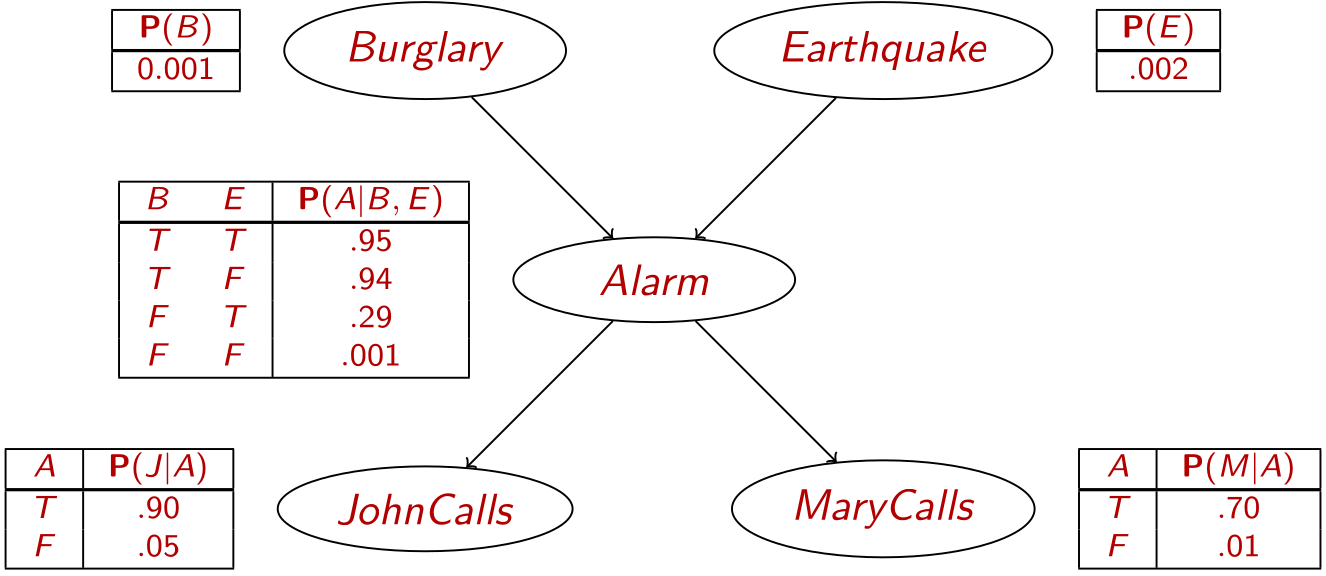
\includegraphics[width=0.75\textwidth]{img/img3.png} \vspace{3.5pt}
    \end{center}
\end{example}

We begin the discussion with a simple toy example, the \textit{student network}.
\begin{example}
    i.e. A student's grade depends on intelligence and on the difficulty of the course.
    SAT scores are correlated with intelligence. A professor writes recommendation letters by only looking at grades. \vspace{3.5pt}

    In this case, our probability space is composed by five relevant random variables: \textit{Difficulty (D)}, \textit{Intelligence (I)}, \textit{SAT score (S)}, \textit{Grade (G)} and \textit{Letter (L)}. \vspace{3.5pt}
    \begin{center}
        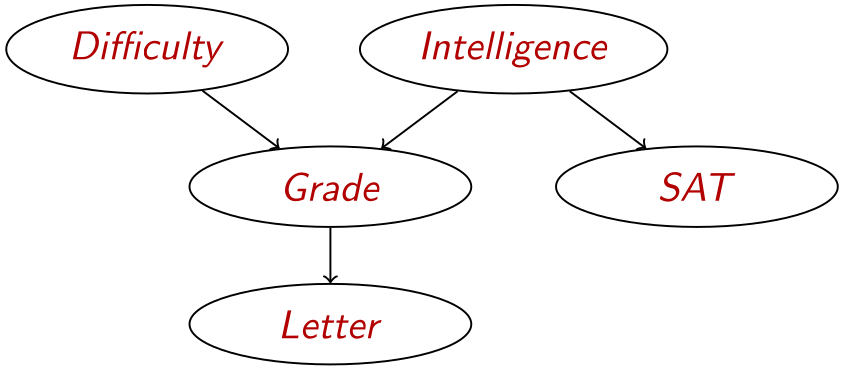
\includegraphics[width=0.5\textwidth]{img/img4.png}
    \end{center} \vspace{3.5pt}
    Consider a particular student, George, that he would like to reason using the student network. We might ask how likely George is to get a strong recommendation from his professor in Analysis.
    Knowing nothing else about George and his grade, this probability is around the $50$ percent. \vspace{3.5pt}

    We now find out that George is not so intelligent. The probability that he gets a strong letter from the professor goes down to 39. We now further discover that Analysis is an easy class.
    The probability that George receive a strong letter is now about 51 percent. \vspace{3.5pt}

    Queries and answers such as this, where we predict the behaviors from causes to effects, are called \textbf{causal reasoning} or \textbf{prediction}\footnote{It reflects the causal direction, from the parent nodes we are just defining which is their influence on their children.}. \vspace{3.5pt}

    Now, assume a recruiter, trying to hire George based on our previous model. By a prior probability, the recruiter believes that George is 30 percent likely to be intelligent. 
    He obtains George's grade record for the class Analysis and sees that George received a low score in that class. His probability that George has high intelligence goes down,
    about 7.9 percent. We note that the probability that the class is a difficult one also goes up, from 40 percent to 62.9 percent. Now, consider that the recruiter lost George's trascript of records, and has only the recommendation letter from George's professor in Analysis, which is weak.
    The probability that George has high intelligence still goes down, but only to 14 percent. Note that if the recruiter has both the grade and the letter, we have the same probability
    as if he had only the grade. \vspace{3.5pt}

    Queries such as this, where we reason from effects to causes, are named \textbf{evidential reasoning} or \textbf{explanation}\footnote{In this case, we are not reasoning from top to bottom, but instead from bottom to top.}. \vspace{3.5pt}

    Finally, George submits his high SAT score to the recruiter. The probability that George has high intelligence goes up dramatically, from 7.9 percent to 57.8 percent. Intuitively, the reason that the SAT score 
    outweights the poor grade is that a student with low intelligence are unlikely to get good scores on their SAT, whereas students with high intelligence can still get C grades in hard class.
    Indeed, we see that the probability that Analysis is a difficult one goes up from 62.9 percent to 76 percent. \vspace{3.5pt} 

    This last pattern is a interesting one. The information about SAT score told us other informations about the student's intelligence, which, in conjuction with the student's grade, gave us some clues about the difficulty of the course. Let examine this pattern in probabilistic terms. \vspace{3.5pt}

    We are saying \vspace{3.5pt}

    $P_s(i^1|g^3) = 0.079$ \vspace{3.5pt}

    On the other hand, if we consider that Analysis is a hard class, we have \vspace{3.5pt}

    $P_s(i^1|d^1, g^3) = 0.11$ \vspace{3.5pt} 

    Here, we are partially explaining why George has got a poor grade. By the way, taking a more tricky example, for instance George got a middle grade in Analysis, we have that \vspace{3.5pt}

    $P_s(i^1|g^2) = 0.175$ \vspace{3.5pt}

    Also if Analysis is a hard class, we get \vspace{3.5pt} 

    $P_s(i^1|d^1, g^2) = 0.34$ \vspace{3.5pt} 

    In effect, we have justified the poor grade via the difficulty of the class. Explaining away is an instance of a general pattern called \textbf{intercasual reasoning},
    where different causes of the same effect, so they are parents of the effect node, can interact.     
\end{example}
\textbf{Compactness} \vspace{3.5pt}

A Bayesian network can often be more \textit{compact} than the full joint distribution. The \textbf{compactness} of a Bayesian network is a property that makes easy to handle
domain with many random variables. \vspace{3.5pt}

At the same time, a Bayesian network grows \textit{linearly}, instead of an \textit{exponential} growth by full joint distribution. Assuming a domain composed by $\mathbf{n}$ Boolean
variables, where each of them is associated with a CPT \textit{(Conditional Probability Table)}\footnote{A CPT for a Boolean variable $\mathbf{X_i}$ with $\mathbf{k}$ parents, has $\mathbf{2^k}$
rows for the combinations of parents values and usually is defined only the True case; the negative case, however $X_i = False$, can be simply computed by the third probability axiom $\mathbf{1 - p}$.}.
If each variable has no more then $\mathbf{k}$ parents, the complete network requires $O(n \times 2^k)$ numbers, as we already know to complete the full joint distribution are necessary
$O(2^n)$.
\begin{example}
    i.e. Comparison of parameters required from the previously example between Bayesian network and full joint distribution. \vspace{3.5pt}

    For the burglar network: \vspace{3.5pt}

    $1 + 1 + 4 + 2 + 2 = 10$ numbers required by the Bayesian network \vspace{3.5pt}

    $2^5 - 1 = 47$ numbers required by the full joint distribution
\end{example}
\textbf{Global semantics} \vspace{3.5pt}

A Bayesian network is a directed acyclic graph with some numeric parameters attached to each node. One way to define what the network means is to define the way in which 
it rapresents a full joint distribution. 
\begin{definition}
    \textbf{Global semantics} defines the full joint distribution as the product of the local conditional distributions:
    \begin{center}
        $P(x_1, ..., x_n) = \prod_{i = 1}^{n} P(x_i|parents(X_i))$
    \end{center}
\end{definition}
\begin{example}
    i.e. 
    
    $P(j, m, a, \neg b, \neg e) \\
    = P(j|a)P(m|a)P(a|\neg b \wedge \neg e)P(\neg b)P(\neg e) \\
    = 0.9 \times 0.7 \times 0.001 \times 0.999 \times 0.998 = 0.000628$
\end{example}
\textbf{Flow of influence} \vspace{3.5pt}

Until now, we used the intuition that edges represent direct dependence. For instance, we said that the letter recommendation from the professor depends only on the student's grade;
this state was encoded by the fact that there is an exit edge from \textit{G} that arrive to \textit{L}. This intuition is \textbf{not} always true. \vspace{3.5pt}

The aim of this section is to understand when we can guarantee independence between random variables. First of all, we begin with a simple case analysis: we try to understand
when a variable \textbf{X} can influence \textbf{Y} given \textbf{Z}. \vspace{3.5pt}

\textbf{Direct connection}. This is the simple case, when X and Y are directly connected via an edge. If X and Y are directly connected, we can always get examples where they 
influence each other, regardless of \textbf{Z}. \vspace{3.5pt}

\textbf{Indirect connection}. Now  we are considering the more complicated case when X and Y are not directly connected, but there is a trail between them. There are four cases
where X and Y are connected via Z. \vspace{3.5pt}
\begin{center}
    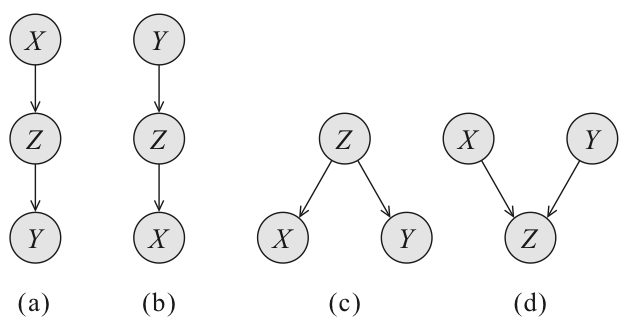
\includegraphics[width=0.6\textwidth]{img/img5.png}
\end{center} \vspace{3.5pt}
The first two correspond to causal chains, the third to a common cause, and the last one to a common effect.

\textbf{(a) Causal trail}. We have a chain like $X \rightarrow Z \rightarrow Y$. X cannot influence Y via Z if Z is observed.

\textbf{(b) Effect trail}. Now we have the same trail but in the opposite direction, so  $Y \rightarrow Z \rightarrow X$. Another time, Y cannot influence X via Z if Z is observed.

\textbf{(c) Common cause}. This type of trail defines the same grade of independence as before. If Z is observed then neither X or Y can influence each other. 

\textbf{(d) Common effect}. In the previously cases, we see a common pattern: if Z is observed then neither X or Y can influence each other. By the way, this kind of trail, 
$X \rightarrow Z \leftarrow Y$, has a new behavior. If Z is not observed influence cannot flow along the trail. So if Z is observed X and Y are independent. In the student example
we analyzed this case, which we called \textit{intercausal reasoning}; we showed that the probability that student has high intelligence goes down when we observe that his grade is 
a poor score, but then goes up when we observe that the class is a hard one. Let us consider a variant of the same case. Assume that we do not observe the student's grade, but we observed
that he received an awful recommendation letter. Intuitively, the same phenomenon happens. The weak letter told us that he received a low grade, and it is sufficient to 
correlate Intelligence and Difficulty.  
\begin{definition}
    If influence can flow from X to Y via Z, the trail $X \longleftrightarrow Z \longleftrightarrow Y$ is \textbf{active}.
\end{definition}
If we consider a longer trail $X_1 \rightarrow \dots \rightarrow X_n$, the first variable $X_1$ can influence the last variable $X_n$, if influence can flow through every single node of the trail.
This will be true if and only if every two-edge trail $X_{i-1} \longleftrightarrow X_i \longleftrightarrow X_{i+1}$ along the trail allows influence to flow.
\begin{definition}
    Let \textbf{Z} be a subset of observed variables. The trail $X_{i-1} \longleftrightarrow X_i \longleftrightarrow X_{i+1}$ is \textbf{active given} Z if
    \begin{itemize}
        \renewcommand{\labelitemi}{-}
        \item $\forall X_{i-1} \rightarrow X_i \leftarrow X_{i+1}$, $X_i$ or one of its descendants are in Z\footnote{The trail reported is the common effect case.}
        \item no other node along the trail is in Z
    \end{itemize}
\end{definition}
However, inside the Bayesian network literacy there is another important notion, named \textbf{d-separation}.
\begin{definition}
    Two sets of nodes \textbf{X}, \textbf{Y} are d-separated given Z if there is no active trail between any $X \in \mathbf{X}$ and $Y \in \mathbf{Y}$ given \textbf{Z}.
\end{definition}
It's possible to summarize few steps to follow to determine if X and Y are independent given Z:
\begin{enumerate}
    \item Mark all nodes in Z or having descendants in Z.
    \item Traverse the graph from X to Y, stopping if we get to a \textbf{blocked} node\footnote{A node is blocked if that node is the middle of an unmarked v-structure \textit{(common effect case)}, or belongs to Z \textit{(cannot be both).}}.
    \item If we can't reach Y, then X and Y are independent.
\end{enumerate}
Another aspects about independence are introduces by the meaning of \textbf{local semantics} and \textbf{Markov blanket}.
\begin{definition}
    \textbf{Local semantics} define that each node is conditionally independent of its \textbf{non-descendants} given its parents\footnote{Here, we are considering the parents of the first node, not the parents of non-descendants.}. 
\end{definition}
\begin{definition}
    Each node is conditionlly independent of all the others nodes given its \textbf{Markov blanket}: so its parents, children and children's parents.
\end{definition}
\label{s_2_2}

\chapter{Bayesian networks}
This paragraph shows how \textbf{informed search strategies} can find solutions more efficiently than \textbf{non-informed search strategies}.

The general approach about informed search strategies is defined by \textbf{best-first search strategy}. Best-first algorithm select a node for the expansion based on an 
\textbf{evaluation function}, briefly written as $f(n)$. Generally, this type of search strategy uses evaluation function as an estimation of the effort required to reach the 
final state; the node with the lowest evaluation is expanded first. \vspace{3.5pt}

The choice of the evaluation function $f(n)$ determines the search strategy. Most best-first algorithms include as a component of $f(n)$ a \textbf{heuristic function}, denoted
$h(n)$. \vspace{3.5pt}
\begin{center}
    $h(n) =$ estimated cost of the path from the current node $n$ to the final state\footnote{Until now, we saw the $g(n)$ function as the path cost from the root node to the
    current state; selecting the node for the expansion with the lowest $g(n)$. Instead the heuristic function $h(n)$ defines the distance from the current node to the final state!}.
\end{center}
We will examine two main applications of the best-first search strategy, which are:
\begin{itemize}
    \renewcommand{\labelitemi}{-}
    \item Greedy best-first search.
    \item A* search.
\end{itemize} 
\label{s_3}

\section{Reasoning patterns}
\textbf{Greedy best-first search} tries always to expand the node closest to the goal state, in a such a way it wanted to build the path that leads to the quickest solution. Thus,
it evaluates nodes by using just the \textit{heuristic function}, $h(n)$. In this case, the \textit{evaluation function} is equal to the \textit{heuristic function}, $f(n) = h(n)$. \vspace{3.5pt}

Let's see how this works for the Romania graph example\footnote{Remember that is always possible to make a tree from a graph, and vice versa.}.
\begin{example}
    i.e. Romania graph, starting from Arad and arriving in Bucharest.
    \begin{center}
        % \includegraphics{Romania graph or tree}
    \end{center}
    We use the \textbf{straight-line distance} heuristic, which we will briefly call $h_{SLD}$. Given Bucharest as the goal state, we must know the straight-line 
    distances to Bucharest. For instance,
    $h_{LSD}(Arad) = 366$. The table below shows each straight-line distance from any given node to Bucharest. \vspace{3.5pt}

    \begin{center}
        \begin{tabular}{|l|p{2cm}|l|p{2cm}|}
            \hline
            \bf Arad & 366 & \bf Mehadia & 241 \\
            \hline
            \bf Bucharest & 0 & \bf Neamt & 234 \\
            \hline
            \bf Craiova & 160 & \bf Oradea & 380 \\
            \hline
            \bf Drobeta & 242 & \bf Pitesti & 100 \\
            \hline
            \bf Eforie & 161 & \bf Rimnicu Vilcea & 193 \\
            \hline
            \bf Fagaras & 176 & \bf Sibiu & 253 \\
            \hline
            \bf Giurgiu & 77 & \bf Timisoara & 329 \\
            \hline
            \bf Hirsova & 151 & \bf Urziceni & 80 \\
            \hline
            \bf Iasi & 226 & \bf Vaslui & 199 \\
            \hline
            \bf Lugoj & 244 & \bf Zerind & 374 \\
            \hline
        \end{tabular}
    \end{center} \vspace{3.5pt}

    Given the table, the first node to be expanded from Arad will be Sibiu, because it is closer to Bucharest than either Zerind or Timisoara. The next node to be expanded
    will be Fagaras because it is closest. Fagaras generated Bucharest, which is the goal. For this problem, greedy best-first search, using the heuristic $h_{LSD}$, finds 
    a solution without ever expanding a node that is not on the solution path. \vspace{3.5pt} 

    \begin{center}
        $\langle Arad, Sibiu, Fagaras, Bucarest\rangle = 450$
    \end{center} \vspace{3.5pt}

    However, the proposed solution is not optimal: the path via Sibiu, Rimnicu Vilcea, Pitesti and Bucharest is lower than the first one. \vspace{3.5pt}

    \begin{center}
        $\langle Arad, Sibiu, Rimnicu, Pitesti, Bucharest\rangle = 418$
    \end{center} \vspace{3.5pt}
\end{example}
This example shows why the algorithm is called \textbf{greedy}, at each step it tries to get as close to the goal as it can. By the way, this search strategy is \textbf{non-optimal}
and may be \textbf{incomplete}, if the data structure presents loopy path. \vspace{3.5pt}

In the worst case, if the depth of the shallowest node is $d$ and the branching factor is $b$, either the time and space complexity will be exponential, $O(b^d)$.
\label{s_3_1}

\chapter{Constructing Bayesian networks}
The basic task for any probabilistic system is to compute the conditional probability distribution for a set of \textbf{query variables}, given some \textbf{evidences}. By the way,
we will consider only one query variable at the time, generally named \textbf{simple query}, that looks like:
\begin{center}
    $\mathbf{P}(X_i|E = e)$
\end{center}
where
\begin{itemize}
    \renewcommand{\labelitemi}{-}
    \item $\mathbf{P}$ is the probability distribution.
    \item $X_i$ defines the query variable, or more simply what we are looking for.
    \item $E = e$ denotes the set of evidence variables, and e is a particular observed event that belongs to one of the random variables.
\end{itemize} \vspace{3.5pt}

We have already seen how to compute posterior probabilities, such as in the burglary network. From the same network, we might ask which is the probability that a 
burglary occured given $JohnCalls$ and $MaryCalls$ true:
\begin{center}
    $\mathbf{P}(Burglary|JohnCalls=True, MaryCalls=True) = \langle 0.284, 0.716 \rangle$
\end{center}
In this section we discuss a smart way for computing this conditional probability without constructing its explict representation.
\label{c_4}
\end{document}